\section{Unstrukturiertes Gitter}
Um generelle Unterschiede zwischen einem strukturierten und unstrukturierten Gitter festzustellen, wurden zusätzlich Berechnungen mit einem unstrukturierten Gitter durchgeführt.

\subsection{Aufgetretene Probleme}
Für den zweiten Stator liegt kein CAD-File, lediglich eine Netzdatei vor. Somit war es nicht möglich ein unstrukturiertes Gitter für diesen zu erstellen. Für die Berechnungen wurde daher das Gitter der Aachen-Turbine teilweise unstrukturiert und strukturiert betrachtet.\\
Die Erstellung der unstrukturierten Gitter war aufgrund von Lizenzproblemen nicht immer möglich, was die Anzahl der durchgeführten Simulationen eingrenzt.
\subsection{Erstellung des Gitters}
Das unstrukturierte Gitter wurde mit Centaur erstellt. Zunächst wurde ein Referenzgitter mit den Standardwerten gebildet. Für das Einstellen von $y^+$ wurde zunächst der gleiche Wandabstand wie im Falle des strukturierten Gitters verwendet. Nach einem ersten Test wurde dieser im Rotor verringert. Die Verteilung von $y^+$ des ersten Stators und Rotors ist in Abbildung \ref{yplusunstrukturiert} dargestellt.
\begin{figure}[htbp]
	\centering
	\includegraphics[width=0.7\textwidth]{yplusunstrukturiert.png}
	\caption{$y^+$ des unstrukturierten Gitters} \label{yplusunstrukturiert}
\end{figure}
\subsubsection{Verwendung von Sources}
Um das Gitter lokal an bestimmten Stellen zu verfeinern wurden  sogenannte Sources mit Hilfe Centaur eingeführt.
Eine davon regelt die unterschiedlichen Wandabstände von Schaufel, Nabe und Gehäuse.\\
Eine weitere Source verfeinert die Zellen im Nachlauf der Schaufel relativ zu den umliegenden Zellen um den Faktor $c = 0.8$.

\subsection{Gitterstudie}
Zuerst wurde der Spalt des Rotors wie beim strukturierten Gitter verfeinert. Anschließend wurde eine Gitterstudie mit verschiedenen Verfeinerungsstufen, siehe Tabelle \ref{tab:verfeinerungenunstrukturiert}, durchgeführt. In den Abbildungen \ref{fig:gitterunstrukturiert1stufe} und \ref{fig:gitterunstrukturiert15stufen} ist der Wirkungsgrad in \% über die Verfeinerungsstufen aufgetragen. Es ist zu erkennen, dass die Wirkungsgrade weiterhin in Abhängigkeit der Kontrollvolumenzahl steigen. Damit eine netzunabhängige Lösung ermittelt werden kann, müssten weitere Verfeinerungsstufen zwischen 2 und 3 und größer 3 gerechnet werden, bis kein Ansteigen oder Absinken mehr zu erkennen ist. Dies war aufgrund von Lizenzproblemen nicht möglich.\\
Für die Berechnungen mit einem temperaturabhängigen $c_p$ und für die Vergleiche mit dem strukturierten Gitter wurde das feinste Netz verwendet.
\begin{table}[h]
		\centering
		\caption{Verfeinerungsstufen des unstrukturierten Gitters}
	\begin{tabular}{ c| c | c| c| c}
Verfeinerungsstufe	&	Stator 1	&		&	Rotor	&		\\
&	Anzahl Knoten	&	Anzahl Elemente	&	Anzahl Knoten	&	Anzahl Elemente	\\
\hline									
0,5	&	61435	&	174098	&	281782	&	724470	\\
1	&	147399	&	473211	&	638948	&	1741931	\\
2	&	244772	&	880367	&	1007020	&	2835297	\\
\textbf{3}	&	\textbf{1196277}	&	\textbf{6457352}	&	\textbf{1880370}	&	\textbf{6844537}	\\

	\end{tabular}
		\label{tab:verfeinerungenunstrukturiert}
\end{table}
\begin{figure}[htbp]
	\centering
	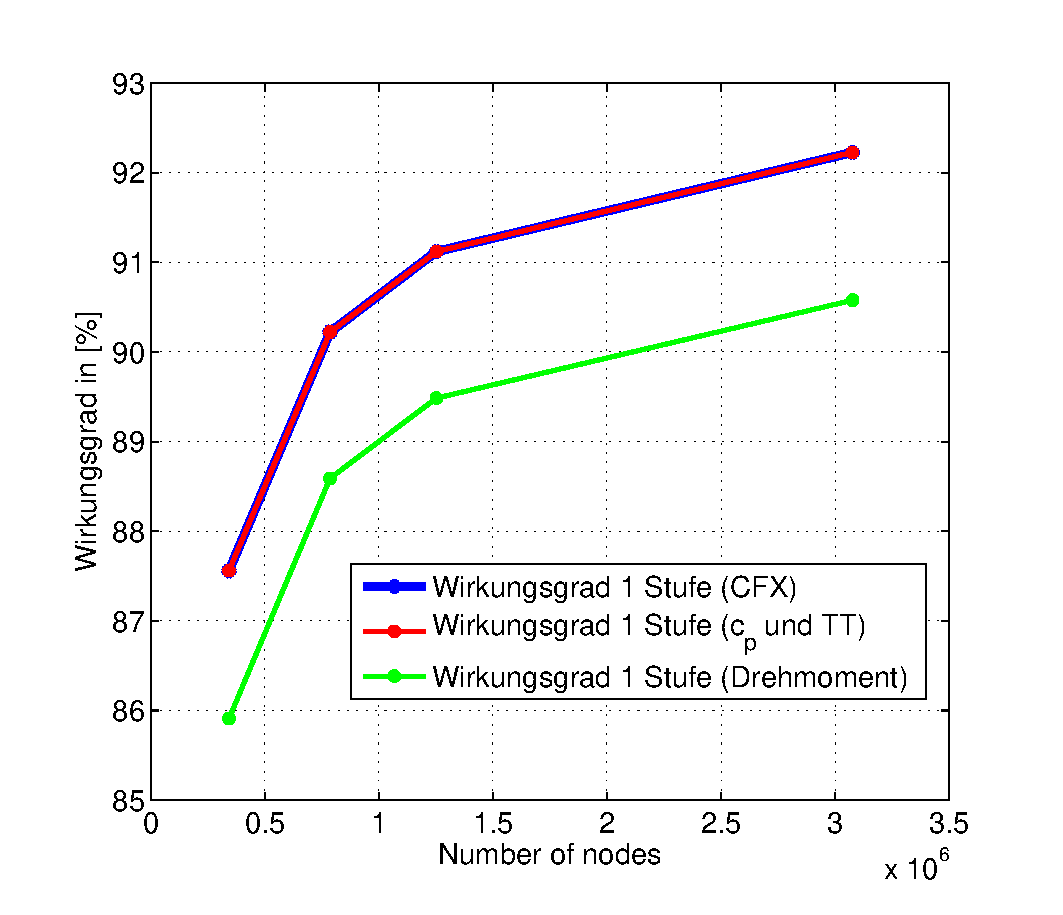
\includegraphics[width=0.7\textwidth]{gitterstudieunstrukturiert1stufe.eps}
	\caption{Gitterstudie des unstrukturierten Gitters für eine Stufe} \label{fig:gitterunstrukturiert1stufe}
\end{figure}

\begin{figure}[htbp]
	\centering
	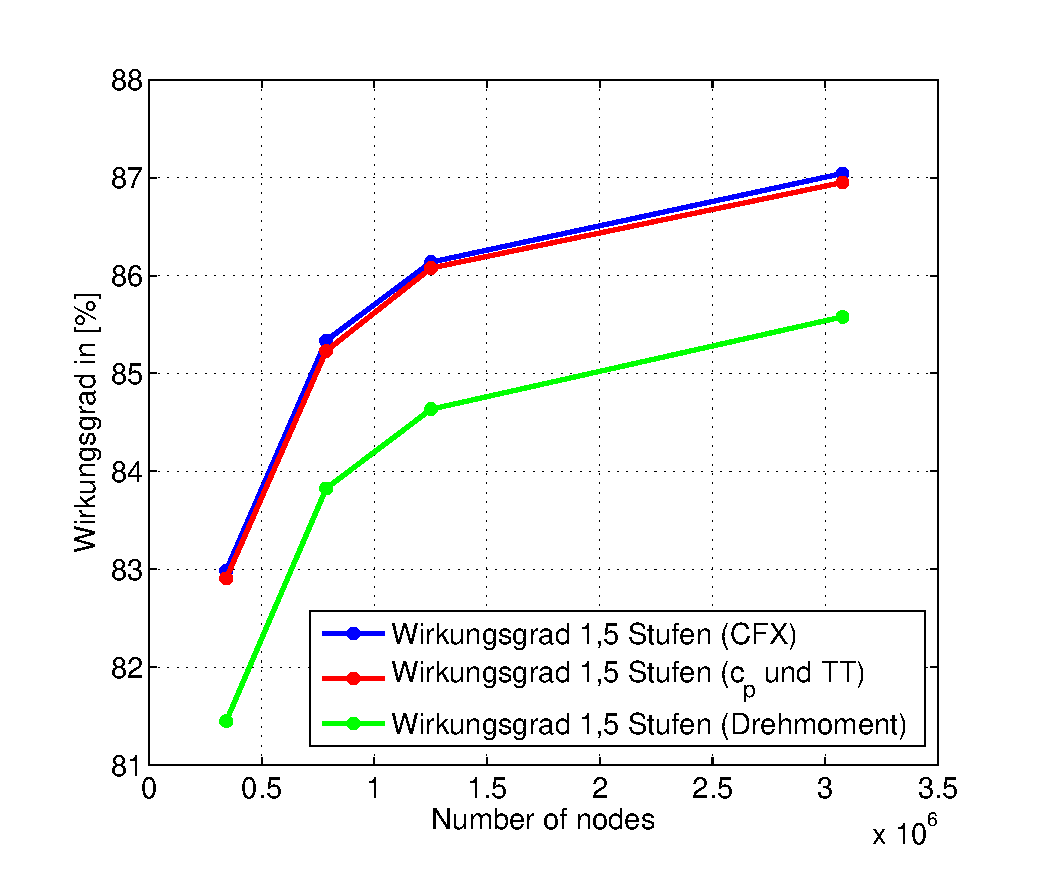
\includegraphics[width=0.7\textwidth]{gitterstudieunstrukturiert15stufen.eps}
	\caption{Gitterstudie des unstrukturierten Gitters für 1,5 Stufen}
	\label{fig:gitterunstrukturiert15stufen}
\end{figure}